% Figure adapted from Del Dotto et al. 2022, Fig. 4(a):
% SPARC_LAB experimental measurement of the beam centroid displacement of a
% long drive bunch as a function of discharge delay Delta t (a proxy for the
% plasma density at beam arrival).  The displacement peaks near Delta t =
% 30 ns where the hose instability (m=1) is dominant, and is suppressed at
% larger delays where self-modulation (m=0) supersedes it.
%
% Data points are approximate digitisations of Fig. 4(a); error bars are the
% reported 1-sigma band over multiple shots.
%
% Build:  pdflatex deldotto_hi_smi.tex
\documentclass[tikz,border=4pt]{standalone}
\usepackage{amsmath}
\usepackage{pgfplots}
\pgfplotsset{compat=1.18}
\usepgfplotslibrary{fillbetween}
\usetikzlibrary{arrows.meta}

\definecolor{datacurve}{RGB}{40, 110, 60}     % measurement curve
\definecolor{bandcol}{RGB}{120, 180, 130}     % error band

\begin{document}
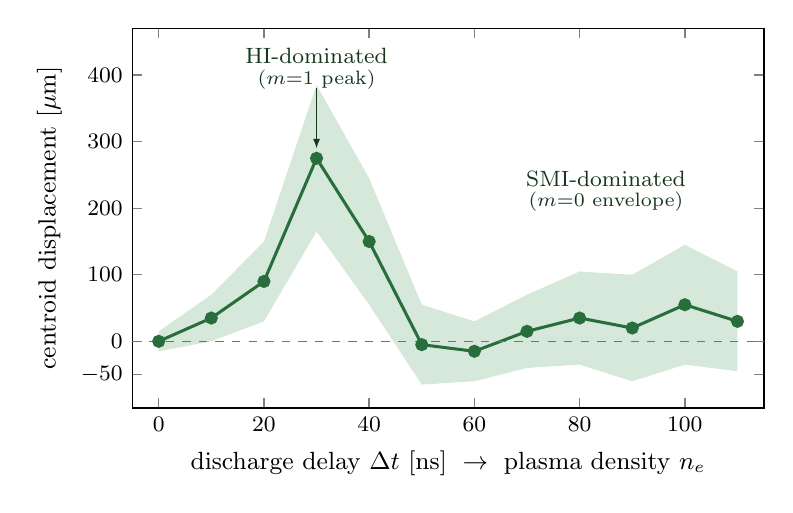
\begin{tikzpicture}

  \begin{axis}[
      width=9.6cm, height=6.4cm,
      xlabel={discharge delay $\Delta t$ [ns] $\;\rightarrow\;$ plasma density $n_e$},
      ylabel={centroid displacement [$\mu$m]},
      xmin=-5, xmax=115,
      ymin=-100, ymax=470,
      xtick={0,20,40,60,80,100},
      ytick={-50,0,100,200,300,400},
      tick align=inside,
      major tick length=0.12cm,
      tick style={line width=0.5pt},
      axis line style={line width=0.6pt},
      label style={font=\small},
      tick label style={font=\footnotesize},
      enlargelimits=false,
      clip=false,
  ]

    % Error band (shaded 1-sigma region)
    \addplot[name path=upper, draw=none, forget plot]
      coordinates {
        (0, 15)   (10, 70)  (20, 150) (30, 385) (40, 245) (50, 55)
        (60, 30)  (70, 70)  (80, 105) (90, 100) (100, 145) (110, 105)
      };
    \addplot[name path=lower, draw=none, forget plot]
      coordinates {
        (0, -15)  (10, 0)   (20, 30)  (30, 165) (40, 55)  (50, -65)
        (60, -60) (70, -40) (80, -35) (90, -60) (100, -35)(110, -45)
      };
    \addplot[bandcol, opacity=0.30, forget plot]
      fill between[of=upper and lower];

    % Measurement data + curve
    \addplot[datacurve, line width=1.1pt,
             mark=*, mark size=1.8pt, mark options={fill=datacurve}]
      coordinates {
        (0, 0)   (10, 35)  (20, 90)  (30, 275) (40, 150) (50, -5)
        (60, -15)(70, 15)  (80, 35)  (90, 20)  (100, 55) (110, 30)
      };

    % Zero baseline (plasma-off reference)
    \addplot[black!55, dashed, line width=0.5pt, forget plot]
      coordinates {(-5, 0) (115, 0)};

    % Regime annotations
    \node[font=\footnotesize, color=datacurve!50!black,
          anchor=north, align=center] at (axis cs:30, 455)
      {HI-dominated\\[-2pt]{\scriptsize($m{=}1$ peak)}};
    \node[font=\footnotesize, color=datacurve!50!black,
          anchor=south, align=center] at (axis cs:85, 180)
      {SMI-dominated\\[-2pt]{\scriptsize($m{=}0$ envelope)}};

    % Thin annotation bracket from HI label to peak
    \draw[-{Latex[length=1.2mm]}, line width=0.4pt, color=datacurve!50!black]
      (axis cs:30, 380) -- (axis cs:30, 290);

  \end{axis}

\end{tikzpicture}
\end{document}
